\subsection{\texorpdfstring{The spaces \(\mathcal{L}_{\mathrm{F}}^{\infty}\)}{The spaces L sub F to infinity}}

DEFINITION 2. --- For every mapping f of X into a Banach space F, one sets \(\mathrm{N}_{\infty}(\mathbf{f}) = \mathrm{M}_{\infty}(|\mathbf{f}|)\) ; f is said to be bounded in measure (for the measure \(\mu\) ) if \(\mathrm{N}_{\infty}(\mathbf{f})\) is finite. The set of mappings of X into F that are measurable and bounded in measure is denoted \(\mathcal{L}_{\mathrm{F}}^{\infty}(\mathrm{X}, \mu)\) (or \(\mathcal{L}_{\mathrm{F}}^{\infty}(\mu)\) , or simply \(\mathcal{L}_{F}^{\infty}\) ).

A function \(\mathbf{f}\) in \(\mathcal{L}_{\mathrm{F}}^{\infty}\) may thus be characterized by the fact that there exists a bounded measurable function equal locally almost everywhere to \(\mathbf{f}\) .

It follows immediately from (1) that

\[
\mathrm{N} _ {\infty} (\mathbf {f} + \mathbf {g}) \leqslant \mathrm{N} _ {\infty} (\mathbf {f}) + \mathrm{N} _ {\infty} (\mathbf {g});
\]

on the other hand, \(\mathrm{N}_{\infty}(\alpha\mathbf{f}) = |\alpha| \mathrm{N}_{\infty}(\mathbf{f})\) for every scalar \(\alpha\) . The set \(\mathcal{L}_{F}^{\infty}\) is therefore a linear subspace of the space of all mappings of X into F, and \(\mathrm{N}_{\infty}(\mathbf{f})\) is a semi-norm on this vector space. Let \((\mathbf{f}_{n})\) be a sequence of functions in \(\mathcal{L}_{F}^{\infty}\) that converges to \(f \in \mathcal{L}_{F}^{\infty}\) for the topology defined by the semi-norm \(\mathrm{N}_{\infty}(\mathbf{f})\) ; for every integer m, there exist a locally negligible set \(H_{m}\) and an integer \(n_{0}\) such that \(|\mathbf{f}(x) - \mathbf{f}_{n}(x)| \leqslant 1/m\) for every integer \(n \geqslant n_{0}\) and every \(x \notin H_{m}\) (every countable union of locally negligible sets being locally negligible); the union H of the \(H_{m}\) is locally negligible, and one sees that \(\mathbf{f}_{n}(x)\) tends uniformly to \(\mathbf{f}(x)\) on the complement of the locally negligible set H; the converse is immediate.

It is clear that every function equal locally almost everywhere to a function in \(\mathcal{L}_{F}^{\infty}\) belongs to \(\mathcal{L}_{F}^{\infty}\) . In particular, the locally negligible functions defined on X with values in F form a linear subspace \(\mathcal{N}_{F}^{\infty}\) of \(\mathcal{L}_{F}^{\infty}\) , characterized by the relation \(\mathrm{N}_{\infty}(\mathbf{f}) = 0\) (the closure of 0 for the topology defined by \(\mathrm{N}_{\infty}(\mathbf{f})\) ). The Hausdorff space associated with \(\mathcal{L}_{F}^{\infty}\) , that is, the quotient space \(\mathcal{L}_{\mathrm{F}}^{\infty}/\mathcal{N}_{\mathrm{F}}^{\infty}\) , is denoted \(\mathrm{L}_{\mathrm{F}}^{\infty}(\mathrm{X}, \mu)\) (or \(\mathrm{L}_{\mathrm{F}}^{\infty}(\mu)\) or \(\mathrm{L}_{\mathrm{F}}^{\infty}\) ); its topology is defined by the norm deduced from \(N_{\infty}\) by passage to the quotient; the norm of a class \(\dot{f} \in L_{F}^{\infty}\) is denoted \(\mathrm{N}_{\infty}(\dot{f})\) , or also \(\|f\|_{\infty}\) . When F = R (resp. C), we write \(\mathcal{L}^{\infty}\) and \(L^{\infty}\) in place of \(\mathcal{L}_{R}^{\infty}\) and \(L_{R}^{\infty}\) (resp. \(\mathcal{L}_{C}^{\infty}\) and \(L_{C}^{\infty}\) ) if this can cause no confusion.

PROPOSITION 2. --- The space \(\mathcal{L}_{\mathrm{F}}^{\infty}\) is complete; the space \(\mathrm{L}_{\mathrm{F}}^{\infty}\) is a Banach space.

For, let \((\mathbf{f}_{n})\) be a Cauchy sequence in \(\mathcal{L}_{F}^{\infty}\) ; for every integer n, there exists an integer \(k_{n}\) such that \(\mathrm{N}_{\infty}(\mathbf{f}_{r}-\mathbf{f}_{s})\leqslant1/n\) for \(r\geqslant k_{n}\) and \(s\geqslant k_{n}\) ; thus, there exists a locally negligible set \(A_{rs}\) such that \(|\mathbf{f}_{r}(x)-\mathbf{f}_{s}(x)|\leqslant1/n\) for all \(x\notin A_{rs}\) . If \(A_{n}\) is the union of the sets \(A_{rs}\) (for \(r\geqslant k_{n}\) and \(s\geqslant k_{n}\) ), then \(A_{n}\) is locally negligible and, for every \(x\notin A_{n}\) , \(|\mathbf{f}_{r}(x)-\mathbf{f}_{s}(x)|\leqslant1/n\) for all indices \(r\geqslant k_{n}\) , \(s\geqslant k_{n}\) . Let A be the locally negligible set formed by the union of the \(A_{n}\) , and set \(\mathbf{g}_{n}(x)=\mathbf{f}_{n}(x)\) for \(x\notin A\) , \(\mathbf{g}_{n}(x)=0\) for \(x\in A\) ; then \(g_{n}\) belongs to \(\mathcal{L}_{F}^{\infty}\) and, by the definition of A, the sequence \((\mathbf{g}_{n})\) converges uniformly on X to a function g. It follows that the function g is measurable (§5, No.~4, Th. 2); moreover, g is bounded on the set of \(x\in X\) where \(|\mathbf{g}_{k_{1}}(x)|\leqslant\mathrm{N}_{\infty}(\mathbf{g}_{k_{1}})\) and, since the complement of this set is locally negligible, g belongs to \(\mathcal{L}_{F}^{\infty}\) . It is clear that in \(\mathcal{L}_{F}^{\infty}\) , the sequence \((\mathbf{g}_{n})\) has limit g, and the same is therefore true of the sequence \((\mathbf{f}_{n})\) , since \(\mathrm{N}_{\infty}(\mathbf{f}_{n}-\mathbf{g}_{n})=0\) for all n.~The second part of the proposition may be deduced immediately from this.

Remarks. --- 1) Every bounded continuous function \(\mathbf{f}\) on \(X\) with values in \(F\) belongs to \(\mathcal{L}_{\mathrm{F}}^{\infty}\) , and

\[
\mathrm{N} _ {\infty} (\mathbf {f}) \leqslant \| \mathbf {f} \| = \sup _ {x \in \mathrm{X}} | \mathbf {f} (x) |.
\]

In order that \(\mathrm{N}_{\infty}(\mathbf{f})=\|\mathbf{f}\|\) for every bounded continuous function f, it is necessary and sufficient that the support of the measure \(\mu\) be equal to X. For, if there exists a continuous function f with negligible compact support and not identically zero, then \(\mathrm{N}_{\infty}(\mathbf{f})=0\) and \(\|f\|>0\) . Conversely, if the support of \(\mu\) is equal to X then, for every bounded continuous function f and every number \(\alpha<\|f\|\) , the set of \(x\in X\) such that \(|\mathbf{f}(x)|>\alpha\) is open and nonempty, hence has outer measure \textgreater0, which shows that \(\mathrm{N}_{\infty}(\mathbf{f})=\|\mathbf{f}\|\) .

When the support of \(\mu\) is equal to \(X\) , we may therefore identify the normed space \(\mathcal{C}^b (X;F)\) , of bounded continuous functions on \(X\) with values in \(F\) , with a subspace of the space \(\mathcal{L}_{F}^{\infty}\) . Since \(\mathcal{L}_F^\infty\) is not in general Hausdorff, the subspace \(\mathcal{C}^b (X;F)\) is not in general closed in \(\mathcal{L}_F^\infty\) , but its canonical image in \(L_F^\infty\) is a closed subspace of \(L_F^\infty\) (which can moreover be identified with \(\mathcal{C}^b (X;F)\) in the case contemplated). In general, \(\mathcal{C}^b (X;F)\) is distinct from \(L_F^\infty\) , that is, for an arbitrary bounded measurable function \(\mathbf{f}\) , there does not in general exist a continuous function \(\mathbf{g}\) equal to \(\mathbf{f}\) locally almost everywhere ( \(\S 5\) , Exer. 12). This implies that the space \(\mathcal{K}(X;F)\) of mappings of \(X\) into \(F\) , continuous with compact support, is in general not dense in \(L_F^\infty\) , whereas it is dense in each of the spaces \(L sub F to the p\) for \(1\leqslant p < +\infty\) ( \(\S 3\) , No.~4. Def. 2).

\pandocbounded{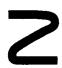
\includegraphics[keepaspectratio]{images/part002_fffac8d3.jpg}}

\begin{enumerate}
\def\labelenumi{\arabic{enumi})}
\setcounter{enumi}{1}
\tightlist
\item
  It is immediate that the topology defined by the semi-norm \(N_{\infty}\) is finer than the topology induced on \(L_{F}^{\infty}\) by the topology of convergence in measure (§5, No.~11).
\end{enumerate}

